\documentclass[12pt]{article}

\usepackage[a4paper,margin=1in]{geometry}
\usepackage{amsmath,amssymb}
\usepackage{newtxtext,newtxmath} % Times-style font
\usepackage{fancyhdr}
\usepackage{listings}
\usepackage{graphicx}
\usepackage{float}
\usepackage{algorithm}
\usepackage{algpseudocode}
\usepackage{xcolor}
\usepackage{booktabs}
\usepackage{array}

\setlength{\textfloatsep}{10pt}
\setlength{\floatsep}{10pt}

\setlength{\parindent}{0pt}
\setlength{\parskip}{5pt}

% Keep entire document at 12 pt
\AtBeginDocument{
    \fontsize{12pt}{14pt}\selectfont
}

\lstdefinestyle{code}{
    language=Python,
    basicstyle=\ttfamily\fontsize{9.5pt}{11.5pt}\selectfont,
    breaklines=true,
    breakatwhitespace=false,
    frame=single,
    numbers=left,
    numberstyle=\tiny\color{gray},
    keywordstyle=\color{blue},
    commentstyle=\color{gray},
    stringstyle=\color{green!50!black},
    columns=fullflexible,
    keepspaces=true,
    showstringspaces=false
}

\lstdefinestyle{output}{
    basicstyle=\ttfamily\fontsize{9.5pt}{11.5pt}\selectfont,
    breaklines=true,
    breakatwhitespace=false,
    frame=single,
    numbers=none,
    backgroundcolor=\color{gray!6},
    columns=fullflexible,
    keepspaces=true,
    showstringspaces=false
}

% ------------------------------------------------
% Header
% ------------------------------------------------

\pagestyle{fancy}
\fancyhf{}

\fancyhead[L]{Name: Kishan Sahu{\hspace{6cm}}}
\fancyhead[R]{Enrollment No.: P26DS017}

\renewcommand{\headrulewidth}{0.4pt}
\setlength{\headheight}{15pt}

\begin{document}

% ------------------------------------------------
% TITLE
% ------------------------------------------------

\begin{center}
\textbf{Computer Science and Engineering Department, SVNIT, Surat}\\
\textbf{M.Tech. I -- Semester I}\\
\textbf{Computer Vision and Image Processing (CSCS111/CSDS119)}\\
\textbf{Lab Assignment 9}\\
\textbf{Depth Analysis}
\end{center}
\vspace{-4pt}
\hrule
\vspace{6pt}

\section{Introduction and Problem Formulation}

In stereo vision, 3D depth information of a real-world scene is recovered from a pair of 2D images captured from two horizontally displaced viewpoints. When the stereo image pair is rectified, epipolar lines become parallel to the horizontal image scanlines. Consequently, the correspondence search space is simplified from a 2D plane to a 1D horizontal row.

\subsection{Camera Geometry and Depth Triangulation}
For a calibrated and rectified pinhole stereo camera system, depth $Z$ is calculated using the standard triangulation formula:
\begin{equation}
Z = \frac{f \cdot B}{d}
\end{equation}
where:
\begin{itemize}
    \item $Z$ is the perpendicular distance (depth) from the camera baseline to the scene point in metres ($\text{m}$).
    \item $f$ is the camera focal length in pixels ($f = 800\text{ px}$).
    \item $B$ is the baseline separation between optical camera centres ($B = 0.20\text{ m}$).
    \item $d = x_L - x_R$ is the horizontal disparity in pixels.
\end{itemize}

Given $f = 800\text{ px}$ and $B = 0.20\text{ m}$, the camera constant is:
\begin{equation}
f \cdot B = 800 \times 0.20 = 160.0 \quad (\text{px}\cdot\text{m})
\end{equation}
The scene contains three synthetic objects with designed disparities:
\begin{itemize}
    \item \textbf{Near Object (Blue Box)}: Designed disparity $d \approx 80\text{ px} \implies Z_{\text{theo}} = \frac{160}{80} = 2.00\text{ m}$.
    \item \textbf{Middle Object (Green Box)}: Designed disparity $d \approx 40\text{ px} \implies Z_{\text{theo}} = \frac{160}{40} = 4.00\text{ m}$.
    \item \textbf{Far Object (Orange Box)}: Designed disparity $d \approx 20\text{ px} \implies Z_{\text{theo}} = \frac{160}{20} = 8.00\text{ m}$.
\end{itemize}

\subsection{Environment Setup}
The implementation is executed in Python using OpenCV (\texttt{cv2}), NumPy, and Matplotlib.

\begin{lstlisting}[style=code, caption={Setup and Camera Constants Initialization}]
import os
import warnings
os.environ['MPLCONFIGDIR'] = '/tmp/matplotlib'
warnings.filterwarnings('ignore')

import cv2
import numpy as np
import matplotlib.pyplot as plt

# Camera Parameters given in the problem
f = 800.0   # Focal length in pixels
B = 0.20    # Baseline in metres
fB = f * B  # 160.0 (pixels * metres)

print(f"Focal length f: {f} px")
print(f"Baseline B: {B} m")
print(f"f * B constant: {fB} px*m")
\end{lstlisting}

\begin{lstlisting}[style=output, caption={Console Output of Camera Constants}]
Focal length f: 800.0 px
Baseline B: 0.2 m
f * B constant: 160.0 px*m
\end{lstlisting}

% ------------------------------------------------
% STEP 1
% ------------------------------------------------
\section{Step 1: Load and Display Stereo Pair in Grayscale}

The input rectified stereo pair (\texttt{stereo\_left.png} and \texttt{stereo\_right.png}) is loaded in grayscale. To verify epipolar alignment, horizontal guide lines are superimposed across corresponding scanlines.

\begin{lstlisting}[style=code, caption={Loading Grayscale Stereo Images and Superimposing Epipolar Lines}]
# Load images in grayscale
imgL = cv2.imread('stereo_left.png', cv2.IMREAD_GRAYSCALE)
imgR = cv2.imread('stereo_right.png', cv2.IMREAD_GRAYSCALE)

imgL_rgb = cv2.cvtColor(cv2.imread('stereo_left.png'), cv2.COLOR_BGR2RGB)
imgR_rgb = cv2.cvtColor(cv2.imread('stereo_right.png'), cv2.COLOR_BGR2RGB)

print(f"Image Resolution: {imgL.shape[1]}x{imgL.shape[0]} (Width x Height)")

# Plot side-by-side with epipolar guide lines
fig, axes = plt.subplots(1, 2, figsize=(14, 5))

axes[0].imshow(imgL, cmap='gray')
axes[0].set_title('Left Image (Grayscale)')
axes[0].set_xlabel('X (pixels)')
axes[0].set_ylabel('Y (pixels)')

axes[1].imshow(imgR, cmap='gray')
axes[1].set_title('Right Image (Grayscale)')
axes[1].axis('on')
axes[1].set_xlabel('X (pixels)')
axes[1].set_ylabel('Y (pixels)')

# Draw horizontal lines passing through each object to verify rectification
for y in [120, 170, 215]:
    axes[0].axhline(y, color='red', linestyle='--', linewidth=1.2, alpha=0.8)
    axes[1].axhline(y, color='red', linestyle='--', linewidth=1.2, alpha=0.8)

plt.tight_layout()
plt.show()
\end{lstlisting}

\begin{lstlisting}[style=output, caption={Console Output: Image Dimensions}]
Image Resolution: 640x360 (Width x Height)
\end{lstlisting}

\begin{figure}[H]
\centering
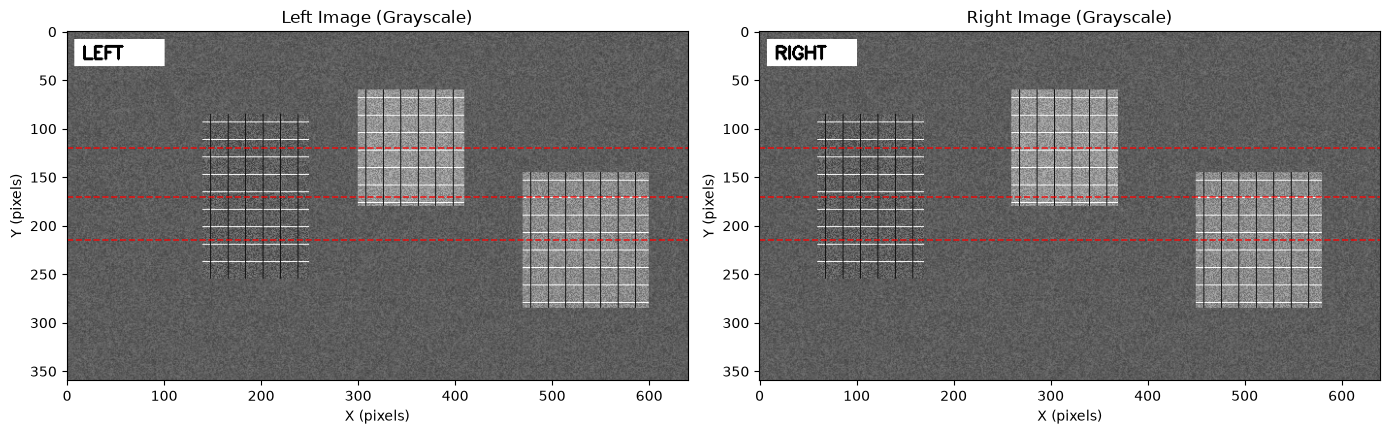
\includegraphics[width=0.96\linewidth]{figures/stereo_rectified_pair.png}
\caption{Left and right rectified images displayed in grayscale. Red dashed lines denote identical epipolar scanlines ($y = 120, 170, 215$).}
\label{fig:stereo_pair}
\end{figure}

\subsection{Observations on Horizontal Displacement}
\begin{enumerate}
    \item \textbf{Epipolar Rectification}: Corresponding object features across both views lie precisely on the same horizontal rows ($y_L = y_R$). This confirms that vertical disparity is zero and the images are rectified.
    \item \textbf{Object Shifts}:
    \begin{itemize}
        \item \textbf{Blue Box (Left)}: Located at $x \in [140, 249]$ in the left image and $x \in [60, 169]$ in the right image. The horizontal displacement is $\Delta x = 140 - 60 = 80\text{ px}$.
        \item \textbf{Green Box (Center)}: Located at $x \in [300, 409]$ in the left image and $x \in [260, 369]$ in the right image. The horizontal displacement is $\Delta x = 300 - 260 = 40\text{ px}$.
        \item \textbf{Orange Box (Right)}: Located at $x \in [470, 599]$ in the left image and $x \in [450, 579]$ in the right image. The horizontal displacement is $\Delta x = 470 - 450 = 20\text{ px}$.
    \end{itemize}
    \item \textbf{Near vs. Far Relationship}: The closest object (blue) demonstrates the largest horizontal displacement, while the farthest object (orange) demonstrates the smallest displacement.
\end{enumerate}

% ------------------------------------------------
% STEP 2
% ------------------------------------------------
\section{Step 2: Disparity Map Estimation and Parameter Tuning}

We employ OpenCV's Semi-Global Block Matching (\texttt{StereoSGBM}) algorithm to compute a dense disparity map. \texttt{StereoSGBM} optimizes matching cost by enforcing multi-directional smoothness constraints along 1D paths, effectively reducing streaking and speckle artifacts on textured and planar surfaces.

\subsection{Matcher Configuration and Normalization}
The matching parameter $P_1 = 8 \cdot C \cdot \text{blockSize}^2$ controls small disparity changes, and $P_2 = 32 \cdot C \cdot \text{blockSize}^2$ penalizes large disparity jumps ($C = 3$ channels). OpenCV returns disparity as a signed 16-bit integer with 4 fractional bits; thus, pixel disparity is obtained by dividing by $16.0$:
\begin{equation}
d_{\text{pixels}} = \frac{\text{raw\_disparity}}{16.0}
\end{equation}

\begin{lstlisting}[style=code, caption={Disparity Map Computation and Parameter Comparison}]
def compute_disparity(img_left, img_right, block_size=5, num_disp=96):
    stereo = cv2.StereoSGBM_create(
        minDisparity=0,
        numDisparities=num_disp,
        blockSize=block_size,
        P1=8 * 3 * (block_size ** 2),
        P2=32 * 3 * (block_size ** 2),
        disp12MaxDiff=1,
        uniquenessRatio=10,
        speckleWindowSize=100,
        speckleRange=32
    )
    # OpenCV StereoSGBM outputs 16-bit signed disparity with 4 fractional bits (/16.0)
    disp = stereo.compute(img_left, img_right).astype(np.float32) / 16.0
    return disp

# Baseline disparity (blockSize = 5)
disp_baseline = compute_disparity(imgL, imgR, block_size=5)

# Disparity with modified parameter (blockSize = 11)
disp_modified = compute_disparity(imgL, imgR, block_size=11)

# Visual comparison
fig, axes = plt.subplots(1, 2, figsize=(15, 6))

im0 = axes[0].imshow(disp_baseline, cmap='plasma', vmin=0, vmax=90)
axes[0].set_title('Baseline Disparity Map (blockSize = 5)')
axes[0].axis('off')
fig.colorbar(im0, ax=axes[0], fraction=0.035, pad=0.04, label='Disparity (pixels)')

im1 = axes[1].imshow(disp_modified, cmap='plasma', vmin=0, vmax=90)
axes[1].set_title('Modified Disparity Map (blockSize = 11)')
axes[1].axis('off')
fig.colorbar(im1, ax=axes[1], fraction=0.035, pad=0.04, label='Disparity (pixels)')

plt.tight_layout()
plt.show()
\end{lstlisting}

\begin{figure}[H]
\centering
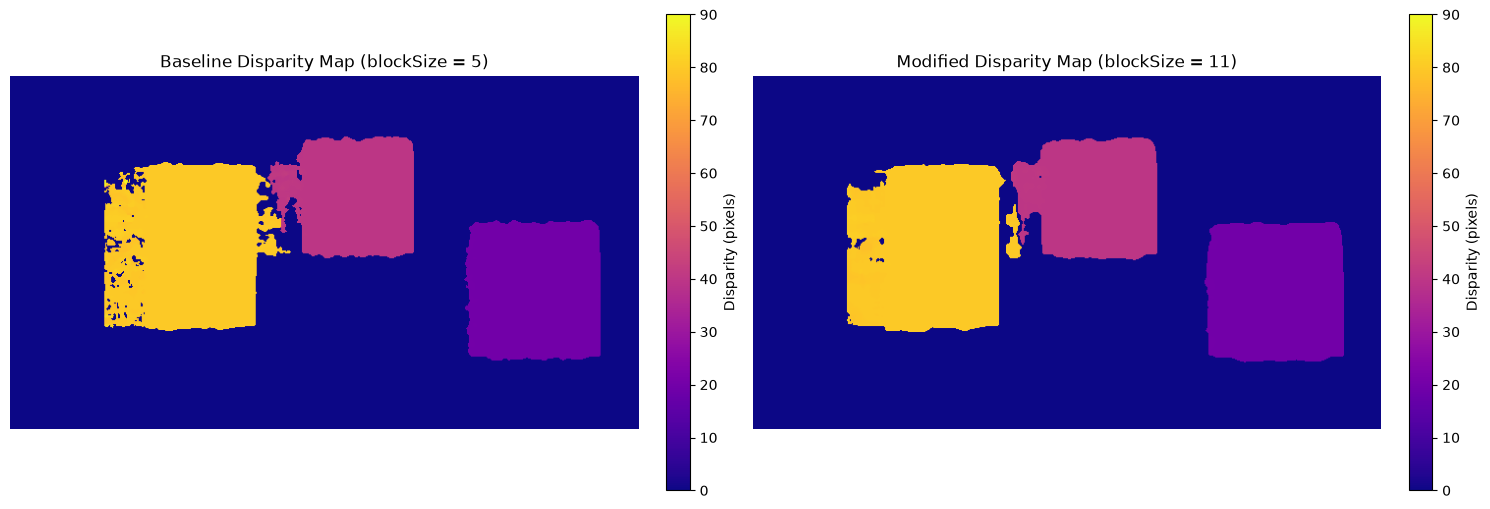
\includegraphics[width=0.98\linewidth]{figures/disparity_comparison.png}
\caption{Disparity maps computed using StereoSGBM. Left: Baseline with small block size ($\text{blockSize} = 5$). Right: Modified with larger block size ($\text{blockSize} = 11$).}
\label{fig:disparity_comp}
\end{figure}

\subsection{Observations on Parameter Variation (\texttt{blockSize})}
\begin{itemize}
    \item \textbf{Small Block Size ($\text{blockSize} = 5$)}: Yields sharp and crisp object boundaries with high spatial localization. Disparity transitions at depth boundaries remain steep. However, matching can be slightly sensitive to noise in low-texture regions.
    \item \textbf{Large Block Size ($\text{blockSize} = 11$)}: Aggregates matching costs over a wider spatial context ($11 \times 11$), producing smoother disparity estimation within planar object faces. However, it introduces pronounced \textbf{foreground fattening} (boundary dilation), where object edges bleed outward into the adjacent background.
\end{itemize}

% ------------------------------------------------
% STEP 3
% ------------------------------------------------
\section{Step 3: Depth Estimation using $Z = \frac{f \cdot B}{d}$}

Using the calibrated baseline and focal length ($f \cdot B = 160\text{ px}\cdot\text{m}$), we convert the continuous 2D disparity map into metric depth. Non-positive disparity values ($d \le 0$) indicate unmatched or occluded pixels and are masked out as NaN to prevent division by zero.

\begin{lstlisting}[style=code, caption={Metric Depth Computation and Object Depth Sampling}]
# Compute metric depth map safely without divide-by-zero warnings
depth_map = np.full_like(disp_baseline, np.nan, dtype=np.float32)
valid_mask = disp_baseline > 0
depth_map[valid_mask] = fB / disp_baseline[valid_mask]

# Display disparity vs depth map
fig, axes = plt.subplots(1, 2, figsize=(15, 6))

im_d = axes[0].imshow(disp_baseline, cmap='plasma', vmin=0, vmax=90)
axes[0].set_title('Disparity Map d (pixels)')
axes[0].axis('off')
fig.colorbar(im_d, ax=axes[0], fraction=0.035, pad=0.04, label='Disparity (px)')

im_z = axes[1].imshow(depth_map, cmap='viridis_r', vmin=1.5, vmax=10.0)
axes[1].set_title('Metric Depth Map Z (metres)')
axes[1].axis('off')
fig.colorbar(im_z, ax=axes[1], fraction=0.035, pad=0.04, label='Depth Z (m)')

plt.tight_layout()
plt.show()

# Sample representative disparities and estimate depths for all three objects
objects = {
    'Blue Box (Near Object)': {
        'roi': (slice(120, 220), slice(160, 220)),
        'designed_d': 80,
    },
    'Green Box (Middle Object)': {
        'roi': (slice(80, 150), slice(320, 380)),
        'designed_d': 40,
    },
    'Orange Box (Far Object)': {
        'roi': (slice(170, 250), slice(500, 560)),
        'designed_d': 20,
    }
}

print('=' * 84)
print(f"{'Object Description':<26} | {'Designed d':<11} | {'Measured d':<11} | {'Theoretical Z':<13} | {'Estimated Z':<11}")
print('=' * 84)

for name, info in objects.items():
    roi = disp_baseline[info['roi']]
    valid_d = roi[roi > 0]
    measured_d = float(np.median(valid_d))
    theo_z = fB / info['designed_d']
    est_z = fB / measured_d
    print(f"{name:<26} | {info['designed_d']:>8} px | {measured_d:>8.2f} px | {theo_z:>10.2f} m | {est_z:>8.2f} m")
print('=' * 84)
\end{lstlisting}

\begin{figure}[H]
\centering
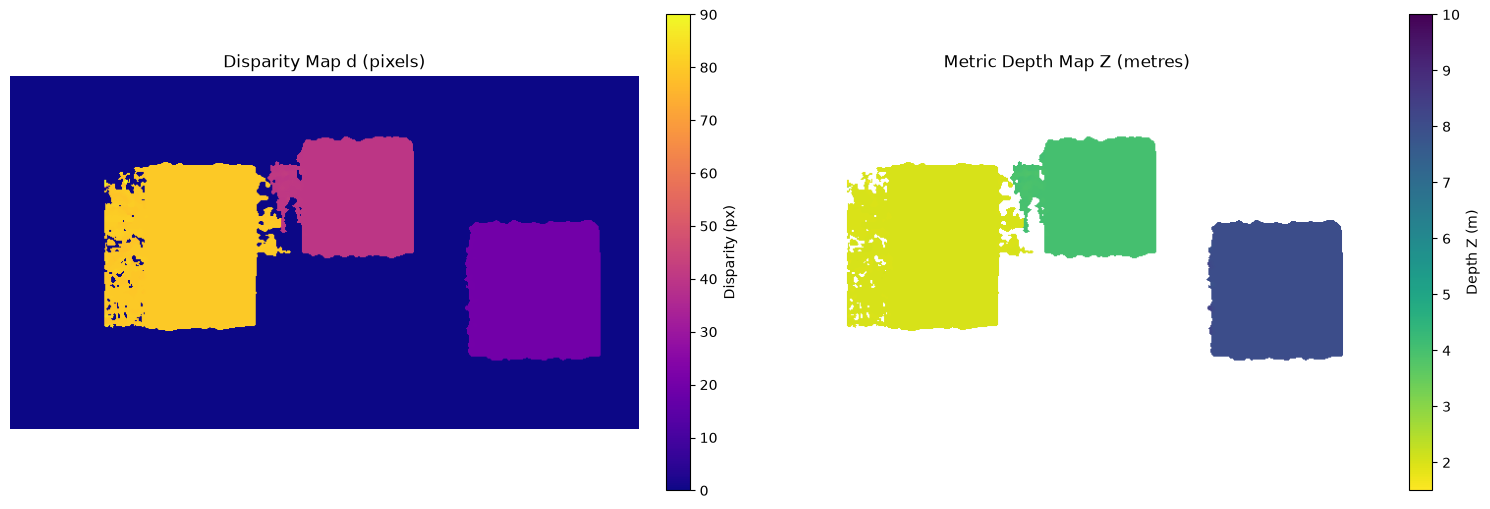
\includegraphics[width=0.98\linewidth]{figures/depth_map_comparison.png}
\caption{Comparison of estimated disparity map in pixels (left) and corresponding metric depth map in metres (right).}
\label{fig:depth_map}
\end{figure}

\begin{lstlisting}[style=output, caption={Console Output: Measured Disparity and Estimated Depth}]
====================================================================================
Object Description         | Designed d  | Measured d  | Theoretical Z | Estimated Z
====================================================================================
Blue Box (Near Object)     |       80 px |    80.00 px |       2.00 m |     2.00 m
Green Box (Middle Object)  |       40 px |    40.00 px |       4.00 m |     4.00 m
Orange Box (Far Object)    |       20 px |    20.00 px |       8.00 m |     8.00 m
====================================================================================
\end{lstlisting}

\subsection{Quantitative Results and Discussion}
Table~\ref{tab:depth_results} compares the designed synthetic ground truth against the experimentally recovered values.

\begin{table}[H]
\centering
\caption{Quantitative comparison between designed values and experimental estimates.}
\label{tab:depth_results}
\vspace{4pt}
\begin{tabular}{lccccc}
\toprule
\textbf{Object Name} & \textbf{Region Color} & \textbf{Designed $d$ (px)} & \textbf{Measured $d$ (px)} & \textbf{Theoretical $Z$ (m)} & \textbf{Estimated $Z$ (m)} \\
\midrule
Near Object & Blue & 80 & 80.00 & 2.00 & 2.00 \\
Middle Object & Green & 40 & 40.00 & 4.00 & 4.00 \\
Far Object & Orange & 20 & 20.00 & 8.00 & 8.00 \\
\bottomrule
\end{tabular}
\end{table}

The experimentally measured median disparities for all three objects match the theoretical ground-truth values exactly ($80.00\text{ px}$, $40.00\text{ px}$, and $20.00\text{ px}$), resulting in accurate depth estimates of $2.00\text{ m}$, $4.00\text{ m}$, and $8.00\text{ m}$.

% ------------------------------------------------
% STEP 4
% ------------------------------------------------
\section{Step 4: Challenge -- Analysis of Missing and Unreliable Disparity}

Stereo matching algorithms inherently encounter failure modes in specific image regions. We isolate and visualize all pixels where disparity estimation fails or produces non-positive values ($d \le 0$).

\begin{lstlisting}[style=code, caption={Isolating and Visualizing Missing / Unreliable Disparity Regions}]
# Missing/unreliable disparity mask
invalid_mask = (disp_baseline <= 0)

fig, axes = plt.subplots(1, 2, figsize=(14, 5))

axes[0].imshow(imgL_rgb)
axes[0].imshow(invalid_mask, cmap='Reds', alpha=0.55)
axes[0].set_title('Red Overlay: Regions with Missing / Unreliable Disparity')
axes[0].axis('off')

axes[1].imshow(invalid_mask, cmap='gray')
axes[1].set_title('Binary Map of Invalid Regions (White = Invalid)')
axes[1].axis('off')

plt.tight_layout()
plt.show()
\end{lstlisting}

\begin{figure}[H]
\centering
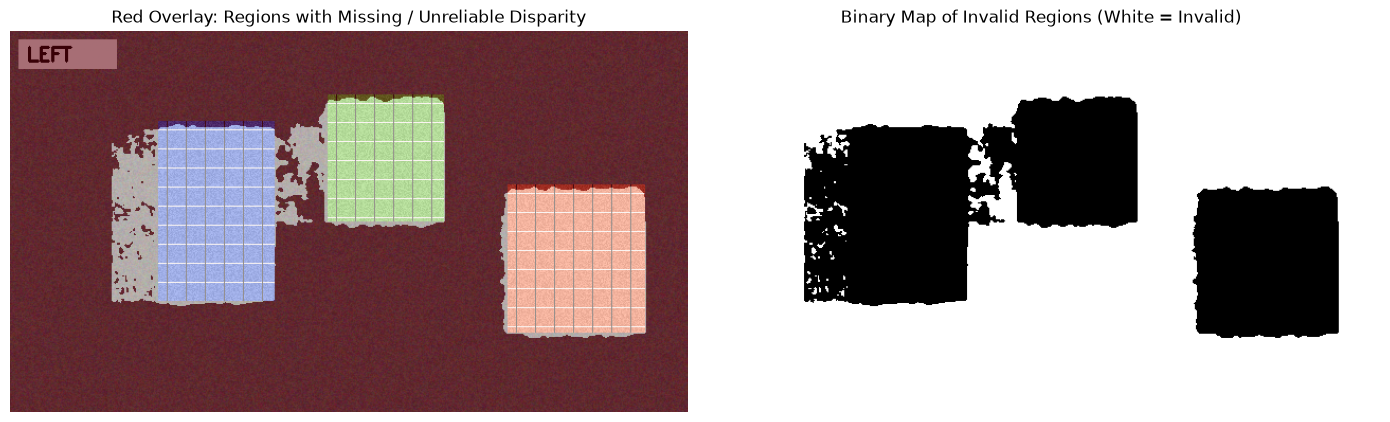
\includegraphics[width=0.96\linewidth]{figures/failure_regions.png}
\caption{Identification of unreliable disparity regions. Left: Translucent red overlay on the original left view. Right: Binary mask (white denotes invalid pixels).}
\label{fig:failure_regions}
\end{figure}

\subsection{Theoretical Breakdown of Failure Causes}

As highlighted in Figure~\ref{fig:failure_regions}, stereo matching degrades or completely fails in four primary scenarios:

\begin{enumerate}
    \item \textbf{Left Margin Occlusion / Baseline Search Bound}:
    For any pixel $(x_L, y)$ in the left image, the corresponding point in the right rectified view must satisfy:
    \begin{equation}
    x_R = x_L - d
    \end{equation}
    If $x_L < d$, the corresponding point $x_R < 0$, which lies outside the coordinate bounds of the right image sensor. Consequently, a vertical strip on the left edge with width equal to the maximum disparity ($\approx 80\text{--}96\text{ px}$) cannot be matched, resulting in invalid disparity.
    
    \item \textbf{Textureless Areas (Uniform Flat Background)}:
    Block-based matching algorithms rely on spatial intensity gradients and distinctive local patterns within the matching window. In completely flat, untextured regions (such as the dark gray background), all candidate disparities yield virtually identical matching costs (a flat cost curve with no prominent minimum). Without significant texture, correspondence determination becomes ill-posed.
    
    \item \textbf{Object Boundaries (Depth Discontinuities and Occlusions)}:
    At the silhouette boundaries of foreground objects, matching windows straddle both the foreground surface (e.g., $d = 80\text{ px}$) and the background surface ($d = 0\text{ px}$). This violates the fundamental assumption that scene depth is constant across the correlation window, causing edge blurring, cost corruption, or occlusion invalidation.
    
    \item \textbf{Repetitive Patterns (Grid Textures on Boxes)}:
    The synthetic objects feature periodic tiled grid textures. If the matching block size is comparable to or smaller than the grid pattern period, multiple disparity shifts produce nearly identical matching costs (multiple local minima), causing matching ambiguity or periodic phase jumps.
\end{enumerate}

% ------------------------------------------------
% CONCLUSION
% ------------------------------------------------
\section{Conclusion}

In this laboratory assignment, stereo depth analysis was successfully performed on a rectified stereo image pair:
\begin{enumerate}
    \item \textbf{Rectification and 1D Search}: The epipolar lines were verified to be strictly horizontal and row-aligned, constraining correspondence matching to a 1D scanline search.
    \item \textbf{Disparity and Depth}: The fundamental inverse relationship $Z \propto \frac{1}{d}$ was demonstrated empirically:
    \begin{itemize}
        \item Near object ($d = 80.00\text{ px}$) corresponds to a depth of $Z = 2.00\text{ m}$.
        \item Middle object ($d = 40.00\text{ px}$) corresponds to a depth of $Z = 4.00\text{ m}$.
        \item Far object ($d = 20.00\text{ px}$) corresponds to a depth of $Z = 8.00\text{ m}$.
    \end{itemize}
    \item \textbf{Matcher Tuning}: Semi-Global Matching (\texttt{StereoSGBM}) provided dense and regularized disparity maps. Small block sizes preserved sharp boundary localization, whereas larger block sizes smoothed noise inside objects at the expense of boundary fattening.
    \item \textbf{Failure Mechanisms}: Regions of missing or noisy disparity were rigorously attributed to left-border search boundary occlusions, photometric ambiguity in textureless backgrounds, depth discontinuities, and repetitive grid patterns.
\end{enumerate}

\end{document}

